% 摸鱼科技 · 摸鱼周报（上市公司年报体例）模板
% A4 单栏，XeLaTeX 编译；页眉页脚为披露文件样式，不是双栏内刊样式。
\documentclass[11pt,a4paper]{article}
\usepackage[usenames]{color}
\usepackage{xcolor}
\definecolor{navy}{HTML}{12345A}
\definecolor{reportred}{HTML}{B02424}
\usepackage{epsfig}
\usepackage{graphics}
\usepackage{graphicx}
\usepackage{caption}
\usepackage{amsmath}
\usepackage{amssymb}
\usepackage{mathtools}
\usepackage{array}
\usepackage{hhline}
\usepackage{url}
\usepackage{geometry}
\geometry{verbose,a4paper,tmargin=20mm,bmargin=18mm,lmargin=18mm,rmargin=18mm}

% 中文支持（需使用 XeLaTeX 编译）
\usepackage{xeCJK}
\setCJKmainfont{Noto Serif CJK SC}         % 正文：思源宋体
\setCJKsansfont{Noto Sans CJK SC}          % 标题：思源黑体
\setCJKmonofont{Noto Sans Mono CJK SC}     % 等宽

\usepackage{fancyhdr}
\pagestyle{fancy}
\fancyhf{}
\lhead{\small\textcolor{navy}{摸鱼科技股份有限公司}}
\rhead{\small 证券代码：002520}
\lfoot{\scriptsize 示意性测算，未经审计 · 文体性戏仿}
\rfoot{\small 第 \thepage 页}
\renewcommand{\headrulewidth}{0.6pt}
\renewcommand{\footrulewidth}{0.3pt}
\renewcommand{\thesection}{第\,\arabic{section}\,节}

\begin{document}

\begin{titlepage}
\centering

\includegraphics[width=0.42\textwidth]{LOGO1.png}\par\vspace{3mm}
{\Large\bfseries\textcolor{navy}{摸鱼科技股份有限公司}\par}
{\small MOYU TECHNOLOGY CO., LTD.\par}
\vspace{1mm}\hrule height 1.2pt\vspace{8mm}
{\Huge\bfseries\textcolor{navy}{这里是摸鱼周报标题，请替换为「XXXX 年第 N 周工作报告」}\par}
\vspace{3mm}{\large\textcolor{reportred}{报告期与周次}\par}
\vspace{6mm}{\small 按上市公司年度报告体例编制 · 文体性戏仿\par}
\vspace{8mm}{\normalsize 这里填写大白话钩子与塞满膨胀名词的经营分析副标题\par}
\vspace{8mm}{\normalsize 报告期：XXXX 年 X 月 X 日 至 X 月 X 日\par}
\vspace{10mm}
% 指标速览：四个 minipage，数值一律来自 model.py 的示意性测算
\begin{minipage}[t]{0.23\textwidth}\centering 指标一\par {\Large\bfseries 7.5 h}\par +11.9\%\end{minipage}\hfill
\begin{minipage}[t]{0.23\textwidth}\centering 指标二\par {\Large\bfseries 22.3\%}\par -4.1 pp\end{minipage}\hfill
\begin{minipage}[t]{0.23\textwidth}\centering 指标三\par {\Large\bfseries 1.444}\par 上限的 89.7\%\end{minipage}\hfill
\begin{minipage}[t]{0.23\textwidth}\centering 指标四\par {\Large\bfseries 41.3\%}\par 协议后 85.2\%\end{minipage}
\vspace{10mm}\par
\begin{minipage}{0.88\textwidth}\small
\textcolor{reportred}{\bfseries 重要提示}\quad
在此填写董事会式免责与数据口径声明：全部指标均为示意性测算、未经审计、
不构成业绩承诺，不指代任何真实企业或个人。
\end{minipage}\par\vfill
\begin{minipage}{0.88\textwidth}\footnotesize\raggedright
编制单位：协同赋能事业部 / 数字效能部\quad 编制人：摸小鱼、明天一定做\\
办公地址：中国 · 摸鱼科技园 B-14 工位\quad 披露日期：XXXX 年 X 月 X 日\\
证券代码：002520\quad 公司简称：摸鱼科技\quad 版本：v0.9
\end{minipage}\par

\includegraphics[height=18mm]{LOGO2.png}
\end{titlepage}
\newpage

\tableofcontents
\newpage

\section{公司基本情况与报告期概览}
这里写报告期内的经营情况、交付物清点与验收口径。
占位占位占位占位占位占位占位占位占位占位占位占位占位占位占位占位占位占位占位占位。

\begin{enumerate}
	\item 交付物一：做什么、谁负责、怎么验收。
	\item 交付物二：做什么、谁负责、怎么验收。
\end{enumerate}

\section{主要指标与统计口径}
这里给出主要经营指标表与逐日工时去向图。

\begin{table}[ht]
	\centering\small
	\caption*{表 1　报告期主要经营指标（示意性测算，未经审计）}
	\begin{tabular}{ m{0.28\textwidth} m{0.15\textwidth} m{0.20\textwidth} m{0.33\textwidth} }
		\hline\hline
		\textbf{指标} & \textbf{本期值} & \textbf{环比} & \textbf{统计口径 / 责任人} \\
		\hline
		会议密度指数 & 7.5 h & +11.9\% & 日历口径 / 本人 \\
		有效产出率 E & 22.3\% & -4.1 pp & 口径 (1) / 本人 \\
		摸鱼熵 H & \textbf{1.444} & +89.7\% 上限 & 口径 (2) / 本人 \\
		\hline\hline
	\end{tabular}
	\par\vspace{1mm}\footnotesize 注：数值由测算模型生成，非真实经营数据。
\end{table}

\begin{figure}[ht]
	\centering
	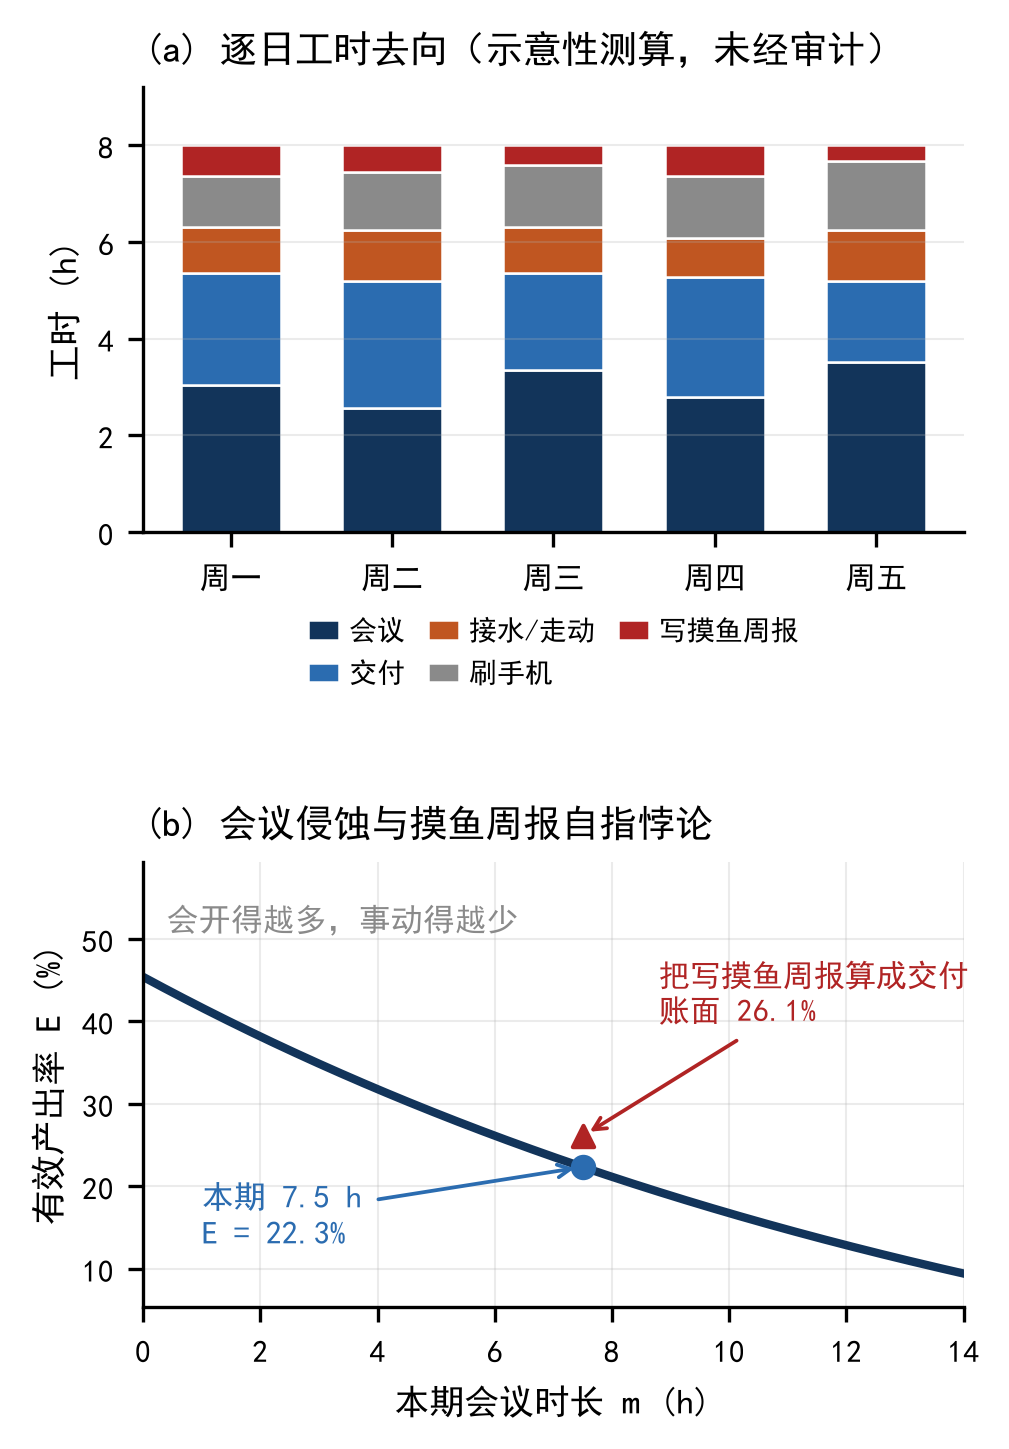
\includegraphics[width=0.82\textwidth]{./fig1.png}
	\caption{逐日工时去向与有效产出率变动（示意性测算曲线，未经审计）。}
\end{figure}

\section{管理层讨论与分析}
\subsection{会议热力学与决策真空}
这里抛招牌黑话、套理论，并给出带定义与编号的口径。

\begin{equation}
	E(m) = E_{0}\,e^{-\lambda m} - \kappa H,\qquad
	H = -\sum_{i=1}^{k} p_{i}\ln p_{i}
	\label{eq:output}
\end{equation}

请确保公式中每个符号都有定义；正文引用「如口径 (1) 所示」。

\subsection{前期比较与同业披露对照}
这里把上期报告半真半假引来逐条对账，既显专业又自然增页。

\section{风险因素与内部控制}
阻塞项按 P0 / P1 / P2 分级，每条带责任人、截止日期与升级路径。

\section{重大事项：摸鱼周报质押协议}
这里郑重介绍一个带牙齿的具体机制：协议 / 制度 / 产品，
有真实代价（押金、罚没、公示）与真实行为学杠杆（承诺装置、损失厌恶、社会可见性）。

\section{下周经营计划与董事会结论}
第一、第二、第三……逐条总结，并给出永久留白的审批签字栏。

\section*{备查文件目录与附录}
\addcontentsline{toc}{section}{备查文件目录与附录}

\noindent\textbf{A. 编制口径与操作规程}\\
这里写示意性测算的操作规程与会议纪要摘录。\\

\noindent\textbf{备查文件}\par
\begin{enumerate}
	\item 《摸鱼科技股份有限公司摸鱼周报管理办法（试行）》，内部制度文件，2026。
	\item 《上期摸鱼周报》，编制人本人，未公开，2026。
\end{enumerate}

\noindent\textit{免责声明：本报告为文体性戏仿，全部指标均为示意性测算、未经审计，
不代表任何真实个人或企业的经营业绩，不构成业绩承诺或管理建议。}

\end{document}
